%	Синтез алгоритмов стабилизации
\section{Синтез алгоритмов стабилизации}

\subsection{Метод модального управления}
Модальное управление - это методы формирования цепей обратных связей, придающих замкнутой системе заранее выбранное расположение корней характеристического уравнения.

Структура модального регулятора задается всегда одинаковой и представляет собой обратную связь по всем переменным состояния. Регулятор линейно преобразует поступившие сигналы, т.е. усиливает и суммирует эти сигналы $x_i$ и выдает в качестве выходы их линейную комбинацию.

Это управление применяется, когда все составляющие вектора состояния объекта управления доступны непосредственному измерению (полная управляемость). 
\begin{equation}
\Dot{x} = A x + B u
\label{eq:main_eq_modal_control}
\end{equation}

Для получения желаемого быстродействия и характеристического уравнения системы введем линейную обратную связь по переменным состояния в соответствии с уравнением
\begin{equation}
u = v - Kx,
\label{eq:eq_control}
\end{equation}

где $v$ - новое обозначение вектора входных воздействий, $u$ - вектор управляющих воздействий с выхода регулятора, $K$ - матрица обратной связи.

$K$ - является матрицей -  строкой, элементы которой - есть коэффициенты обратных связей по всем составляющим вектора $x$.
$$K = \left[ K_1 K_2 ... K_n \right]$$.

Структурная схема исходной системы с обратной связью по переменным состояния приведена на рис.~(\ref{fig:struct_scheme_feedback_variable_sost})

\begin{figure}[h]
	\centering
	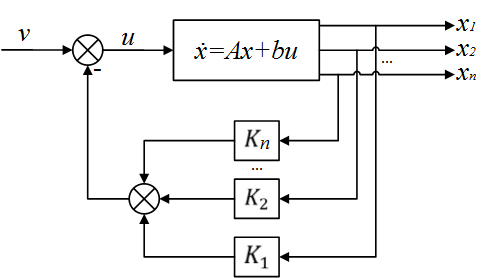
\includegraphics[scale=0.6]{images/struct_scheme_feedback_variable_sost.png}
	\caption{Структурная схема системы с обратной связью по переменным состояния}
	\label{fig:struct_scheme_feedback_variable_sost}
\end{figure}



Задача распределения корней характеристического уравнения замкнутой системы желаемым образом обеспечивает устойчивость заданной стабилизации и ее желаемую динамику быстродействия, перерегулирования и
т.п.

Рассмотрим линейный объект $\Dot{x} = Ax + Bu$ в форме пространства состояния.

В данном случае вектор $x$ включает в себя параметры угла и угловой скорости соответственно по каналам управления, $u$ - управление соответствующее приведенным моментам или силам действующее на летательный аппарат по рассматриваемому каналу.

Целью управления является 
$$||x(t) -  x^{*}(t)|| \rightarrow 0, \  t \rightarrow \infty, $$

где $x^{*}(t)$ - желаемая динамика замкнутой системы заданной эталонной модели.

Решение поставленной задачи методом модального управления находим в виде линейной обратной связи по составленному ОУ и заданному воздействию эталонной модели $\Dot{x}_{*}$.
\begin{equation}
\Dot{x}_{*} = A_{*} x_{*} + B_{*} u_{*},
\label{eq:ur_mod_contol_with_star}
\end{equation}
где 
$$A_{*} = \begin{pmatrix}
0 & 1 \\
- \alpha^{*}_0 & - \alpha^{*}_1 \end{pmatrix} \ B = \begin{pmatrix}0 \\ \alpha^{*}_0 \end{pmatrix}$$

Управляющее воздействие $u = K x + K_r y_{*}$.

Компоненты вектора $K = \begin{pmatrix} K_1 \\ K_2 \end{pmatrix}$ и скалярного коэффициента усиления $K_r$ определяется из соотношения:
\begin{equation}
BK = A_{*} - A
\label{eq:ur_mod_control_BK}
\end{equation}
\begin{equation}
BK_r = B
\label{eq:ur_mod_control_BKr}
\end{equation}

Решение первого матричного уравнения существует если матрицы $A$ и $A^{*}$ согласованы по структуре, а ОУ является управляемым, то есть выполняется условие:
\begin{equation}
\label{eq:usl_upr}
rang \left( B | AB|...|A^n B\right) = n
\end{equation}

В рассматриваемом случае это условие соответствует выполнению следующих условий:

\begin{equation}
\label{eq:usl_this_1}
det \left( B|AB\right) \neq 0
\end{equation}

Уравнения для определения $K_r$ должно быть разрешенным относительно $K_r$ при структурной согласованности $B$ и $B^{*}$.

\clearpage

\subsection{Постановка задачи слежения по ЦМ}
Для того чтобы использовать вышеприведенный метод мы преобразуем исходную модель в форме пространства состояния с учетом того, что $u_{\xi}$, $u_{\eta}$, $u_{\zeta}$ - моменты по каналам.

\begin{equation}
\label{eq:norm_slej}
|| x_i(t) - x_i^{\text{эм}} (t) || \leq \overline{\Delta}_{xi}, \ \forall t \geq T_{*},
\end{equation}
где $x_i^{\text{эм}}$ - траектория эталонной модели заданной в виде:
\begin{equation}
\label{eq:ur_etalon_traektor}
\Dot{x}_i^{\text{эм}} = A_{*i} x_i^{\text{эм}} + B_{*i} r_{*i},
\end{equation}
где $x_1 = (\xi \dot{\xi})^T$, $x_2 = (\eta \dot{\eta})^T$, $x_3 = (\zeta \dot{\zeta})^T$, $i = \overline{1, 3}$, $i$ - номер канала, $u_i$ - управление.
$$u_1 = u_{\xi}, \  u_2 = u_{\eta}, \ u_3 = u_{\zeta}$$
$$r_{*1} = \xi_{*} (t), \ r_{*2} = \eta_{*} (t), \ r_{*3} = \zeta_{*} (t).$$

Приведенная выше формализация позволяет уйти от исходной системы к системе, описанной выше и использовать метод модального управления. 

Желаемое качество отработки задается спектром матрицы эталонной модели: $\lambda_{*j}(A_{*i}):Re \lambda_{*j} < 0$ (устойчивость), с заданым расположением корней.

Задаем расположение корней так, чтобы ближайший к мнимой оси полюс задавал быстродействие системы, если он вещественный, то будет апериодическое движение, если будет пара ближайших к мнимой  комплексно-сопряженных корней, то колебательное движение.

Исходя из того, что у нас система 2-го порядка выбирались 2 полюса так чтобы из требований времени второй полис был отнесен дальше от мнимой оси, чтобы его динамика не сильно сказывалась

Точность определеяем выбором параметром матрицы $B_{*}$ так, чтобы статическая ошибка была равна 1.
\clearpage

\subsection{Результаты моделирования переходных процессов}
\clearpage

\subsection{Результаты моделирования системы стабилизации ЦМ}
\clearpage